% This is samplepaper.tex, a sample chapter demonstrating the
% LLNCS macro package for Springer Computer Science proceedings;
% Version 2.20 of 2017/10/04
%
\documentclass[runningheads]{llncs}
%
\usepackage{graphicx}
% Used for displaying a sample figure. If possible, figure files should
% be included in EPS format.
%
% If you use the hyperref package, please uncomment the following line
% to display URLs in blue roman font according to Springer's eBook style:
% \renewcommand\UrlFont{\color{blue}\rmfamily}

\usepackage{amsmath}

\begin{document}
%
\title{Global optimization method with numerically calculated function derivatives\thanks{Supported by Russian Foundation for Basic Research (grant 19-07-00242)}}
%
\titlerunning{Global optimization method with numerical derivatives}
% If the paper title is too long for the running head, you can set
% an abbreviated paper title here
%
\author{Victor Gergel\orcidID{0000-0002-4013-2329} \and Alexander Sysoyev\orcidID{0000-0003-1542-7624}}
	%\inst{1}\orcidID{0000-1111-2222-3333} \and
%Second Author\inst{2,3}\orcidID{1111-2222-3333-4444} \and
%Third Author\inst{3}\orcidID{2222--3333-4444-5555}}
%
\authorrunning{V. Gergel, A. Sysoyev}
% First names are abbreviated in the running head.
% If there are more than two authors, 'et al.' is used.
%
\institute{Lobachevsky State University of Nizhny Novgorod,\\ Nizhny Novgorod, Russian Federation\\
	\email{alexander.sysoyev@itmm.unn.ru, gergel@unn.ru}}
	% \and
%Springer Heidelberg, Tiergartenstr. 17, 69121 Heidelberg, Germany
%\email{lncs@springer.com}\\
%\url{http://www.springer.com/gp/computer-science/lncs} \and
%ABC Institute, Rupert-Karls-University Heidelberg, Heidelberg, Germany\\
%\email{\{abc,lncs\}@uni-heidelberg.de}}
%
\maketitle              % typeset the header of the contribution
%
\begin{abstract}
The paper proposes a method for solving computationally time-consuming multidimensional global optimization problems. The developed method combines the use of a nested dimensional reduction scheme, numerical estimates of the objective function derivatives, and optimization schemes for discontinuous functions. Derivatives significantly reduce the cost of solving global optimization problems, however, the use of a nested scheme can lead to the fact that the derivatives of the reduced function become discontinuous. Typical global optimization methods are highly dependent on the continuity of the objective function. Thus, to use derivatives in combination with a nested scheme, an optimization method is required that can work with discontinuous functions. The paper discusses the corresponding method, as well as the results of numerical experiments confirming the applicability of the described approach.

\keywords{Multidimensional optimization \and Global search algorithms \and Lipschitz condition \and Numerical estimations of derivative values \and Dimensionality reduction \and Discontinuous functions \and Numerical experiments.}
\end{abstract}
%
%
%
\section{Introduction}

The global (or multiextremal) unconstrained optimization problem \cite{Floudas1996,Floudas2016,Horst1990,Locatelli2013,Pardalos2016,Paulavicius2014,Pinter1996,Strongin1978,Strongin2000,Strongin2013,Zhigljavsky2008} can be stated as follows
\begin{equation}
\label{eq:problem_statement}
\varphi(y^*) = \min\{\varphi(y)\colon y \in D\},
\end{equation}
where search domain $D$ represents an $N$-dimensional hyperinterval:
\[
D = \{y \in \bbbr^N\colon a_i \leq y_i \leq b_i,\; i = \overline{1,N}\}.
\]

The objective function $\varphi(y)$ is assumed to be a multiextremal one. Also one of the commonly used assumptions is that the minimized function satisfies the Lipschitz condition
\begin{equation}
\label{eq:Lipschitz_for_function}
|\varphi(y_2) - \varphi(y_1)| \leq L \|y_2 - y_1\|,\; y_1, y_2 \in D.
\end{equation} 
where $L > 0$ is the Lipschitz constant, and $\| \cdot \|$ denotes the Euclidean norm in $\bbbr^N$.

The Lipschitz condition corresponds to the assumption of a limited variation of the function value at limited variations of its parameters. This condition allows making the estimates of potential behaviour of the function $\varphi(y)$ based on a finite set of its values computed at some points in the search domain $D$.

To solve problem (1) numerically, optimization methods usually generate a sequence of points $y_k$, which converges to the global optimum $y^*$. The amount of computation can grow exponentially with an increase in the number of variable parameters $N$.

One approach to reduce computational costs is to use differentiability of the objective function. In this case the fulfilment of the Lipschitz condition (2) may be expanded onto the partial derivatives $\varphi_i^\prime(y), 1 \leq i \leq N$ of the objective function as well i.e.
\begin{equation}
\label{eq:Lipschitz_for_derivative}
|\varphi_i^\prime(y_2) - \varphi_i^\prime(y_1)| \leq L_i \|y_2 - y_1\|,\; y_1, y_2 \in D, 1 \leq i \leq N,
\end{equation} 
where $L_i > 0, 1 \leq i \leq N$ are the corresponding Lipschitz constants for the partial derivatives $\varphi_i^\prime(y), 1 \leq i \leq N$~\cite{Baritompa1994,Breiman1993,Gergel1996,Gergel1997,Gergel2017,Lera2013,Sergeyev1998,Sergeyev2015,Shpak1995}.

However, in some applied optimization problems the computing of the derivatives may be restricted or even impossible. In this case the usage of the global optimization methods, in which the necessary values of derivatives are computed numerically may be useful~\cite{Gergel2017,Goryachih2017,Griewank2008,Nocedal2006}.

A widely used approach to solve the problem of multidimensional optimization is to reduce it to one-dimensional. This reduction may be based on using Peano (space-filling) curves~\cite{Piyavskij2006,Strongin2000}, the nested multistep reduction scheme~\cite{Dam2010,Shi2000}, the diagonal generalization technique~\cite{Gergel1997,Pinter1996,Sergeyev2015}, etc. As a result, one-dimensional optimization algorithms can be effectively applied in the multidimensional case~\cite{Baritompa1994,Breiman1993,Dam2010,Galperin1985,Gergel1996,Gergel2017}. It is known that using the nested multistep reduction scheme can lead for executing some redundant global search iterations~\cite{Dam2010,Shi2000,Strongin2000}. This deficiency can be diminished by using the values of derivatives of the objective function -- see the results of numerical experiments given in section 5.

In this paper, the global optimization algorithm utilizing the numerical derivatives of the objective function $\varphi(y)$ is considered. In Section 2, the base one-dimensional algorithm utilizing the numerical derivatives is given. Section 3 introduces a nested dimension reduction scheme that allows one to generalize the proposed one-dimensional algorithm to solving multidimensional global optimization problems. Section 4 describes an approach of usage derivatives in combination with a nested scheme, that can work with discontinuous functions. In Section 5, the results of the numerical experiments are considered, which confirm the developed approach to be promising.

\section{One-dimensional Global Optimization Algorithm Utilizing Numerical	Derivatives}\label{sec:GOAND}

The proposed optimization algorithm is based on the adaptive global method using derivatives (AGMD) ~\cite{Gergel1996,Gergel1997}, designed to solve one-dimensional global optimization problems

\begin{equation}
\label{eq:problem_statement_1d}
\varphi(x^*) = \min\{\varphi(x)\colon x \in [a,b]\}.
\end{equation} 

The adaptive global method using numerical derivatives (AGMND) is a modification of AGMD, in which the values of the first derivative of the objective function are replaced by their numerical estimates ~\cite{Gergel1997,Goryachih2017}.

Consider the computational scheme of the AGMND. The first two iterations are performed at the boundary points $a$ and $b$. Then let $k, k > 1$ iterations of the global search were completed, and the values of the objective function $\varphi(x)$ have been computed at each iteration (hereinafter, these computations will be called \textit{trials}). The test point of the next ($k+1$) optimization iteration is determined by the following rules.

\textbf{Rule 1.} Renumber the points of previous trials by subscripts in increasing order

\begin{equation}
a = x_0 < x_1 < \ldots < x_i < \ldots < x_k = b.
\end{equation} 

\textbf{Rule 2.} Compute the numerical estimations of the first derivatives of $\varphi(x)$ at the points of the executed search iterations $x_i, 0 \le i \le k$ according to the expressions:
\begin{equation}
\dot{z}_i = \left\lbrace
\begin{array}{lr}
\frac{z_{i+1}-z_i}{x_{i+1}-x_i}, i = 0, \\
\frac{z_i-z_{i-1}}{x_i-x_{i-1}}, 1 \le i \le k,
\end{array}
\right.
\end{equation}
hereinafter $z_i, 0 \le i \le k$ denotes $\varphi(x_i)$.

\textbf{Rule 3.} Compute the estimation of the Lipschitz constant from (\ref{eq:Lipschitz_for_derivative}) for the first derivative of the optimized function
\begin{equation}\label{m}
m = \left\{
\begin{array}{ll}
rM, & M > 0, \\
1, & M = 0,
\end{array}
\right.
\end{equation}
where
\begin{equation}
M = \max(M_{i}), 1 \le i \le k, 
\end{equation}
\begin{equation}
M_{i} = \max \left\{
\begin{array}{ll}
|\dot{z}_i-\dot{z}_{i-1}| / |x_i-x_{i-1}|, \\
-2[z_i-z_{i-1}-\dot{z}_{i-1}(x_i-x_{i-1})] / (x_i-x_{i-1})^2|, \\
2[z_i-z_{i-1}-\dot{z}_i(x_i-x_{i-1})] / (x_i-x_{i-1})^2|,
\end{array}
\right.
\end{equation}
and $r > 1$ is the reliability parameter of the algorithm.

\textbf{Rule 4.} Compute the characteristic $R(i)$ for each interval $(x_{i-1}, x_i), 1 \le i \le k$ according to the following expressions to estimate the minimum possible values of $\varphi(x)$ in the interval ($(x_{i-1}, x_i)$
\begin{equation}
R(i) = \left\{
\begin{array}{ll}
\widehat{\varphi}_i(\widehat{x_i}), & \widehat{x_i} \in [\bar{x}_i,\bar{\bar{x}}_i], \\
\min (\widehat{\varphi}_i(\bar{x}_i),\widehat{\varphi}_i(\bar{\bar{x}}_i)), & \widehat{x_i} \notin [\bar{x}_i,\bar{\bar{x}}_i],
\end{array}
\right.
\end{equation}
where
\begin{equation}
\widehat{x_i} = \frac{-\dot{z}_{i-1}+m(\bar{x}_i-x_{i-1})+mx_i}{m},
\end{equation}
and the auxiliary functions (minorants) $\widehat{\varphi}_i(x), 1 \le i \le k$ take the form
\begin{equation}\label{phi_hat}
\widehat{\varphi}_i(x) = \left\{
\begin{array}{ll}
\widehat{\varphi}_{i1}(x) = z_{i-1}+\dot{z}_{i-1}(x_i-x_{i-1})-0.5m(x-x_{i-1})^2, & x \in (x_{i-1},\bar{x}_i) \\
\widehat{\varphi}_{i2}(x) = A_i(x-\bar{x}_i)+0.5m(x-\bar{x}_i)^2 +B_i, & x \in [\bar{x}_i, \bar{\bar{x}}_i], \\
\widehat{\varphi}_{i3}(x) = z_i-\dot{z}_i(x-x_i)-0.5m(x-x_i)^2, & x \in (\bar{\bar{x}}_i, x_i],
\end{array}
\right.
\end{equation}
where
\begin{equation}
\begin{array}{lr}
A_i=\dot{z}_{i-1}-m(\bar{x}_i-x_{i-1}), \\
B_i = \widehat{\varphi}_{i1}(\bar{x}_i), \\
\bar{x}_i = \frac{(z_{i-1}-\dot{z}_{i-1}x_{i-1})-(z_i-\dot{z}_ix_i)+m(x_i^2-x_{i-1}^2)/2-md_i^2}{m(x_i-x_{i-1})+(\dot{z}_i-\dot{z}_{i-1})} \\
\bar{\bar{x}}_i = \frac{(z_{i-1}-\dot{z}_{i-1}x_{i-1})-(z_i-\dot{z}_ix_i)+m(x_i^2-x_{i-1}^2)/2+md_i^2}{m(x_i-x_{i-1})+(\dot{z}_i-\dot{z}_{i-1})} \\
d_i = (x_i-x_{i-1})/2-(\dot{z}_i-\dot{z}_{i-1})/2m.
\end{array}
\end{equation}

Each characteristic $R(i), 1 \le i \le k$ calculated in this way is an estimation of the minimum possible value of the minorant $\widehat{\varphi}_i(x)$ from (\ref{phi_hat}) in the intervals $[x_{i-1}, x_i]$ and the estimation of the minimum possible values of $\varphi(x)$ in these intervals.

\textbf{Rule 5.} Find the interval $(x_{t-1}, x_t)$ with the minimal characteristic $R(t)$

\begin{equation}\label{R_t}
R(t) = \min \{R(i) : 1 \le i \le k\}.
\end{equation}

In the case when there are several intervals satisfying (\ref{R_t}), for definiteness, the interval with the minimum number $t$ is taken.

\textbf{Rule 6.} Compute the next point of the next trial $x^{k+1}$ accordingly

\begin{equation}\label{key}
x^{k+1} = \left\{
\begin{array}{ll}
\widehat{x}_t, & \widehat{x}_t \in [\bar{x_t},\bar{\bar{x}}_t], \\
\bar{x}_t, & \widehat{\varphi}(\bar{x}_t) \le \widehat{\varphi}(\bar{\bar{x}}_t), \\
\bar{\bar{x}}_t, & \widehat{\varphi}(\bar{x}_t) > \widehat{\varphi}(\bar{\bar{x}}_t).
\end{array}
\right.
\end{equation}

The stopping condition is defined by the following relation
\begin{equation}
|x_t-x_{t-1}| \le \varepsilon,
\end{equation}
where $\varepsilon$ is the accuracy, $\varepsilon > 0$.
The minimum computed value of the objective function is accepted as the current estimate of the global minimum value i.e:

\begin{equation}
\varphi^* = \min \{z_i : 0 \le i \le k\}.
\end{equation}

\textbf{Note 1.} The computing of the numerical estimations $\dot{z}_i, 0 \le i \le k$ of the first derivative of the function $\varphi(x)$ can be performed also using the three-point approximating expressions:
\begin{equation}
\dot{z}_i = \left\{
\begin{array}{ll}
\frac{1}{H_1^2}
\left( -(2+\delta_2)z_0+\frac{(1+\delta_2)^2}{\delta_2}z_1-\frac{1}{\delta_2}z_2 \right), & i = 0, \\
\frac{1}{H_i^{i+1}}
\left( -\delta_{i+1}z_{i-1}+\frac{\delta_{i+1}^2-1}{\delta_{i+1}}z_i+\frac{1}{\delta_{i+1}}z_{i+1}
\right), & 1 < i < k, \\
\frac{1}{H_{k-1}^k}
\left(
\delta_k z_{k-2}-\frac{(1+\delta_k)^2}{\delta_k}z_{k-1}+\frac{(2\delta_k+1)}{\delta_k}z_k
\right), & i = k,
\end{array}
\right.
\end{equation}
where $H_i^{i+1} = h_i+h_{i+1}, \delta_{i+1} =\frac{h_{i+1}}{h_i}$ and $h_i=x_i-x_{i-1}$, see~\cite{Griewank2008}.
These formula used three points of trials, and can be used in the \textbf{Rule 2} if $k > 2$.

\textbf{Note 2.} For the applicability of the computational scheme described above, the fulfilment of the following inequalities
\begin{equation}\label{note2}
x_{i-1} < \bar{x}_i < \bar{\bar{x}}_i < x_i
\end{equation}
for all intervals $(x_{i-1}, x_i), 1 \le i \le k$ is necessary. If the estimate of the Lipschitz constant $m$ computed in (\ref{m}) is insufficient and the condition (\ref{note2}) is violated for some $1 \le i \le k$ the value $m$ should be refined. Thus, the maximum root of the equations
\begin{equation}
\left\{
\begin{array}{ll}
-(z_i-z_{i-1})+0.5(\dot{z}_i+\dot{z}_{i-1})+0.25m(x_i-x_{i-1})^2-\frac{(\dot{z}_i-\dot{z}_{i-1})^2}{4m}=0, \\
(z_i-z_{i-1})-0.5(\dot{z}_i+\dot{z}_{i-1})+0.25m(x_i-x_{i-1})^2-\frac{(\dot{z}_i-\dot{z}_{i-1})^2}{4m}=0 ,
\end{array}
\right.
\end{equation}
was selected as $m$ in this case for AGMD~\cite{Gergel1996}.


\section{Nested Dimensionality Reduction Scheme}\label{sec:nestedreduction}

One approach to solve multidimensional optimization problems is dimension reduction, which allows to use effective one-dimensional optimization methods. In this paper, dimension reduction is performed using the well-known nested scheme~\cite{Dam2010,Shi2000,Strongin1978,Strongin2000,Strongin2013}. According to this scheme, the solving of a multidimensional optimization problem (\ref{eq:problem_statement}) can be obtained by solving a series of nested one-dimensional problems:

\begin{equation}
\min \{ \varphi(y) : y \in D\} = \min_{[a_1,b_1]} \ldots \min_{[a_N,b_N]} \varphi(y_1, \ldots, y_N).
\end{equation}

In other words the solving of problem (\ref{eq:problem_statement}) is reduced to solving a one-dimensional problem:
\begin{equation}\label{eq:nested}
\varphi(y^*) = \min_{y \in D} = \min_{y_1 \in [a_1,b_1]}\widetilde{\varphi}_1(y_1),
\end{equation}
where
\begin{equation}\label{eq:nested1}
\begin{array}{c}
\widetilde{\varphi}_i(y_i)=\varphi_i(y_1, \ldots, y_i) = \min\limits_{y_{i+1} \in [a_{i+1},b_{i+1}]}\varphi_i(y_1, \ldots, y_i,y_{i+1}), 1 \le i \le N, \\ \\
\widetilde{\varphi}_N(y_1, \ldots, y_N) = \varphi(y_1, \ldots, y_N).
\end{array}
\end{equation}

The one-dimensional function in (\ref{eq:nested}) is constructed according to a general recursive scheme -- in order to compute the values $\widetilde{\varphi}_1(y_1)$ for some given value of the variable
$y_1 = \widehat{y_1}$ it is necessary to minimize the function

\begin{equation}
\widetilde{\varphi}_2(y_2) = \varphi_2(\widehat{y}_1,y_2).
\end{equation}

With respect to $y_2$ the function $\widetilde{\varphi}_2(y_2)$ is a one-dimensional one as well since the value of the variable $y_1$ is given and fixed one. Next, in turn, in order to compute the value of $\widetilde{\varphi}_2(y_2)$ at the point $y_2 = \widehat{y2}$, it is necessary to minimize the function
\begin{equation}
\widetilde{\varphi}_3(y_3) = \varphi_3(\widehat{y}_1,\widehat{y}_2,y_3),
\end{equation}
and so forth.

Additional information on the nested dimensionality reduction scheme and its applications for solving the multidimensional global optimization problems can be found, for example, in~\cite{Dam2010,Shi2000,Strongin2000,Strongin2013}.


\section{Global Optimization Algorithm for Discontinuous Functions}\label{sec:GOADF}

To solve problem (\ref{eq:problem_statement}), the method with derivatives can only be used if the objective function is smooth. But one-dimensional functions $\widetilde{\varphi}_i(y_i), 1 \le i < N$ from (\ref{eq:nested1}) (except the function of the
last decomposition level $\widetilde{\varphi}_N(y_N)$) in the nested reduction scheme can be non-smooth at some points i.e. the derivatives of these functions can be discontinuous at these points.

Strictly speaking, the AGMND method described in Section 2 can only be used to minimize one-dimensional function $\widetilde{\varphi}_N(y_N)$) at the last level of decomposition. The paper~\cite{Gergel2019} presents the results of experiments comparing a number of optimization methods, which showed that the AGMND method provides good efficiency even in the case of nonsmooth reduced functions. But with increasing the problem dimensionality ($N$) the number of discontinuity points of the derivatives can grow exponentially and increase the number of executed trials.

To handle the discontinuity problem one can use the combined method which uses AGMND to minimize the one-dimensional function $\widetilde{\varphi}_N(y_N)$) and any one-dimensional method without derivatives for the remaining functions $\widetilde{\varphi}_i(y_i), 1 \le i < N$.

Another way is to use an optimization method that can work with discontinuous functions. As such a method, the paper considers the modified Strongin algorithm~\cite{Strongin1990}. Consider its computational scheme.

The first iteration is performed at any point in the interval $(a, b)$. Then let $k, k > 1$ iterations of the global search were completed. The test point of the next ($k+1$) optimization iteration is determined by the following rules.

\textbf{Rule 1.} Renumber the points of previous trials by subscripts in increasing order

\begin{equation}
a = x_0 < x_1 < \ldots < x_i < \ldots < x_k = b.
\end{equation}

\textbf{Rule 2.} Compute

\begin{equation}
\mu_i = \frac{|z_i-z_{i-1}|}{|x_i-x_{i-1}|}, 1 \le i \le k.
\end{equation}

\textbf{Rule 3.} Reorder $\mu_i$ values in descending order

\begin{equation}
\mu(1) > \mu(2) > \ldots > \mu(k)
\end{equation}
and determine a minimal number $p$ such that 

\begin{equation}\label{eq:p}
\frac{\mu(p)}{\mu(p+1)} \ge Q, 1 \le p < qk,
\end{equation}
where $q$ and $Q$ are given numbers ($0 < q < 1 < Q$). 

Construct a subset of numbers

\begin{equation}
J = \{i: 1 \le i \le k, \mu_i = \mu(j), 1 \le j \le p \}
\end{equation}
of those intervals to which sufficiently large $\mu_i$ correspond.

\textbf{Rule 4.} Set for all intervals

\begin{equation}
\delta_i = \left\{
\begin{array}{ll}
sign(z_i-z_{i-1}), & i \in J, \\
0, & i \notin J,
\end{array}
\right. 1 \le i \le k.
\end{equation}

\textbf{Rule 5.} Compute the estimation of the Lipschitz constant

\begin{equation}
\mu = \max(\mu_{i}), 1 \le i \le k
\end{equation}
and the characteristic $R(i)$ for each interval $(x_{i-1}, x_i), 1 \le i \le k$

\begin{equation}
R(i) = (1+|\delta_i|)\Delta_i+(1-|\delta_i|)\frac{(z_i-z_{i-1})^2}{(r\mu)^2\Delta_i}-2\frac{(1-\delta_i)z_i+(1+\delta_i)z_{i-1}}{r\mu},
\end{equation}
where $\Delta_i = x_i - x_{i-1}$.

\textbf{Rule 6.} Find the interval $(x_{t-1}, x_t)$ with the maximal characteristic $R(t)$

\begin{equation}
R(t) = \max \{R(i) : 1 \le i \le k\}.
\end{equation}

\textbf{Rule 7.} Compute the next point of the next trial $x^{k+1}$ accordingly

\begin{equation}
x^{k+1} = \frac{x_t+x_{t-1}}{2}-(1-|\delta_t|)\frac{z_t-z_{t-1}}{2r\mu}.
\end{equation}

\section{Results of Numerical Experiments}\label{sec:results}

Paper~\cite{Gergel2019} presents the results of comparing the Brent Algorithm (BA)~\cite{Brent1973}, the Strongin Algorithm (GSA)~\cite{Strongin1978,Strongin2000}, GSA algorithm with the dimensionality reduction using Peano space-filling curves~\cite{Strongin1978} (GSA-Peano), AGMD, AGMND and two combined methods (GSA-D and GSA-ND). In the last two methods, GSA was applied to optimize the reduced one-dimensional functions $\widetilde{\varphi}_1(y_1)$ from (\ref{eq:nested1}).

A family of well-known two-dimensional multiextremal test functions~\cite{Strongin1978,Strongin2000,Strongin2013} defined by the relations:
\begin{equation}\label{eq:grish}
\begin{gathered}
\varphi(y_1,y_2)=-\left\{
\Bigl(\sum_{i=1}^7\sum_{j=1}^7\left[A_{ij}a_{ij}(y_1,y_2)+B_{ij}b_{ij}(y_1,y_2)\right]\Bigr)^2+\right.\\
\left.+\Bigl(\sum_{i=1}^7\sum_{j=1}^7\left[C_{ij}a_{ij}(y_1,y_2)+D_{ij}b_{ij}(y_1,y_2)\right]\Bigr)^2\right\}^{\frac{1}{2}},\\
a_{ij}(y_1,y_2)=\sin(\pi i y_1)\sin(\pi j y_2),\\
b_{ij}(y_1,y_2)=\cos(\pi i y_1)\cos(\pi j y_2),
\end{gathered}
\end{equation}
where $0 \le y1, y2 \le 1$, were used. The values $-1 \le A_{ij}, B_{ij}, C_{ij}, D_{ij} \le 1$ are the independent random generated parameters distributed uniformly over the interval $[-1, 1]$.

In all these methods, an adaptive scheme of computing the reliability parameter $r$ from (\ref{m}) was applied: $r=3+10/k$ where $k$ is the number of executed trials. The accuracy of solving the optimization problems was $\varepsilon = 0.001$. In order to obtain the reliable
results, 100 multiextremal problems (\ref{eq:grish}) were solved in every series of experiments.

These results demonstrated the AGMND method to show the best performance (the smallest number of trials).

Thus, to evaluate the efficiency of the scheme described in the section \ref{sec:GOADF}, further experiments were carried out only with the AGMND and GSA-ND methods. In the last method, the modified Strongin algorithm was applied to optimize the reduced one-dimensional functions $\widetilde{\varphi}_1(y_1)$ from (\ref{eq:nested1}).

From the experimental results, the operational characteristics of the compared methods were constructed. The operational characteristic is a graph of the number of solved problems (the ordinate axis) vs the number of executed trials (the abscissa axis)~\cite{Strongin1978,Strongin2000,Strongin2013}. The operational characteristics of the compared methods are presented in Fig.~\ref{fig1}.

\begin{figure}
	\centering
	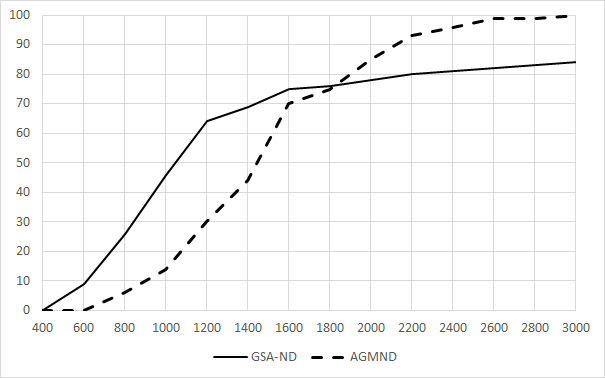
\includegraphics[width=0.75\linewidth]{fig1.png}
	\caption{Operational characteristics of the compared optimization methods. The vertical axis is the percentage of problems solved with the required accuracy, the horizontal axis is the number of executed trials} \label{fig1}
\end{figure} 

As shown GSA-ND with discontinuous modification achieved $100\%$ solvability later than AGMND, but GSA-ND solved $75\%$ of problems faster than AGMND. The results of the numerical experiments allow us to conclude that the proposed approach is quite promising, but additional studies are necessary.

\section*{Conclusion}\label{sec:conclusion}

In this paper, an efficient method for solving computationally time-consuming multidimensional global optimization problems is proposed.

The developed method combines nested dimension reduction scheme, numerical estimation of the derivatives of the objective function, and discontinuous function optimization schemes.

The developed method combines the use of a nested dimensional reduction scheme, numerical estimates of the objective function derivatives, and optimization schemes for discontinuous functions. Derivatives significantly reduce the cost of solving global optimization problems, however, the use of a nested scheme can lead to the fact that the derivatives of the reduced function become discontinuous. Typical global optimization methods are highly dependent on the continuity of the objective function. Thus, to use derivatives in combination with a nested scheme, an optimization method is required that can work with discontinuous functions. The paper discusses the corresponding method, as well as the results of numerical experiments confirming the applicability of the described approach.



%
\begin{thebibliography}{8}

\bibitem{Baritompa1994}
Baritompa W.: Accelerations for a variety of global optimization methods. Journal of Global Optimization, \textbf{4} 37--45 (1994).

\bibitem{Breiman1993}
Breiman L. and Cutler A.: A deterministic algorithm for global optimization. Mathematical Programming, \textbf{58} 179--199 (1993).

\bibitem{Brent1973}
Brent R.P.: Algorithms for Minimization Without Derivatives. Englewood Cliffs NJ: Prentice-Hall (1973).

\bibitem{Dam2010}
Dam E.R., Husslage B. and Hertog D.: One-dimensional nested maximin designs, Journal of Global Optimization \textbf{46}, 287--306 (2010).

\bibitem{Floudas1996}
Floudas C.A. and Pardalos M.P.: State of the Art in Global Optimization. Computational Methods and Applications. Dordrecht: Kluwer Academic Publishers (1996).

\bibitem{Floudas2016}
Floudas C.A. and Pardalos M.P.: Recent Advances in Global Optimization. Princeton University Press (2016).

\bibitem{Galperin1985}
Galperin E.A.: The cubic algorithm. Journal of Mathematical Analysis and Applications \textbf{112}, 635--640 (1985).

\bibitem{Gergel1996}
Gergel V.P.: A method of using derivatives in the minimization of multiextremum functions. Computational Mathematics and Mathematical Physics, \textbf{36} 729--742 (1996) (In Russian).
	
\bibitem{Gergel1997}
Gergel V.P.: A global optimization algorithm for multivariate function with Lipschitzian first derivatives. Journal of Global Optimization, \textbf{10}  257--281 (1997).

\bibitem{Gergel2017}
Gergel V.P. and Goryachih A.S.: Global optimization using numerical approximations of derivatives, Learning and Intelligent Optimization. In: LION 2017. Lecture Notes in Computer Science 10556, 320--325 (2017).

\bibitem{Gergel2019}
Gergel V. and Goryachih A.: Multidimensional global optimization using numerical estimates of objective function derivatives. In: Optimization Methods and Software (2019).

\bibitem{Goryachih2017}
Goryachih A.S. and Rachinskaya M.A.: Multidimensional global optimization method using numerically calculated derivatives. Procedia Computer Science \textbf{119}, 90--96 (2017).

\bibitem{Griewank2008}
Griewank A. and Walther A.: Evaluating Derivatives: Principles and Techniques of Algorithmic Differentiation. SIAM (2008).

\bibitem{Horst1990}
Horst R. and Tuy H.: Global Optimization: Deterministic Approaches. Springer-Verlag (1990).

\bibitem{Lera2013}
Lera D. and Sergeyev Y.D.: Acceleration of univariate global optimization algorithms working with Lipschitz functions and Lipschitz first derivatives. SIAM Journal on Optimization, \textbf{23}, 508--529 (2013).

\bibitem{Locatelli2013}
Locatelli M. and Schoen F.: Global Optimization: Theory, Algorithms, and Applications. SIAM (2013).

\bibitem{Nocedal2006}
Nocedal J. and Wright S.: Numerical Optimization. Springer (2006).

\bibitem{Pardalos2016}
Pardalos M.P., Zhigljavsky A.A. and \u{Z}ilinskas J., Advances in Stochastic and Deterministic
Global Optimization, Springer, 2016.

\bibitem{Paulavicius2014}
Paulavi\u{c}ius R. and \u{Z}ilinskas J.: Simplicial Global Optimization. Springer Briefs in Optimization. Springer (2014).

\bibitem{Pinter1996}
Pint\'{e}r J.D.: Global Optimization in Action (Continuous and Lipschitz Optimization: Algorithms, Implementations and Applications). Kluwer Academic Publishers (1996).

\bibitem{Piyavskij2006}
Piyavskij S.: An algorithm for finding the absolute extremum of a function. Computational Mathematics and Mathematical Physics \textbf{12}, 57--67 (1972) (In Russian).

\bibitem{Sergeyev1998}
Sergeyev Y.D.: Global one-dimensional optimization using smooth auxiliary functions. Mathematical Programming \textbf{81}, 127--146 (1998).

\bibitem{Sergeyev2015}
Sergeyev Y.D.: A deterministic global optimization using smooth diagonal auxiliary functions. Communications in Nonlinear Science and Numerical Simulation \textbf{21}, 99--111 (2015).

\bibitem{Shi2000}
Shi L. and \'{O}lafsson S.: Nested partitions method for global optimization. Operations Research \textbf{48}, 390--407 (2000).
	
\bibitem{Shpak1995}
Shpak A.: Global optimization in one-dimensional case using analytically defined derivatives of objective function. Computer Science Journal of Moldova \textbf{3}, 168--184 (1995).

\bibitem{Strongin1978}
Strongin R.G.: Numerical Methods in the Multiextremal Problems (information-statistical algorithms). Nauka (1978) (In Russian).

\bibitem{Strongin1990}
Strongin R.G.: Search of global optimum. Znanie (1990) (In Russian).

\bibitem{Strongin2000}
Strongin, R.G., Sergeyev, Ya.D.: Global Optimization with non-convex constraints: sequential and parallel algorithms. Dordrecht: Kluwer Academic Publishers. (2000, 2nd ed. 2013, 3rd ed. 2014)

\bibitem{Strongin2013}
Strongin R.G., Gergel V.P., Grishagin V.A. and Barkalov K.A.: Parallel Computations in the Global Optimization Problems. MSU Publishing (2013) (In Russian).

\bibitem{Zhigljavsky2008}
Zhigljavsky A. and \u{Z}ilinskas A.: Stochastic Global Optimization. Springer, Berlin (2008).

\end{thebibliography}


\end{document}
